
%	Documentação do Trabalho Prático 1 de AEDSIII
%	@Sandro Miccoli
%
%	* Você pode identificar erros de grafia através do seguinte comando linux:
%		aspell --encoding="utf-8" -c -t=tex --lang="pt_BR" tp1.tex
%

\documentclass[12pt]{article}
\usepackage{sbc-template}
\usepackage{graphicx}
\usepackage{latexsym}
\usepackage{changepage}   % for the adjustwidth environment
\usepackage{subfigure}
\usepackage{times,amsmath,epsfig}
\usepackage{graphicx,url}
 \makeatletter
 \newif\if@restonecol
 \makeatother
 \let\algorithm\relax
 \let\endalgorithm\relax
\graphicspath{{./data/}}
\usepackage[lined,algonl,ruled]{algorithm2e}
\usepackage{multirow}
\usepackage[brazil]{babel}
\usepackage[utf8]{inputenc}
\usepackage{listings}

\usepackage{alltt}
\renewcommand{\ttdefault}{txtt}

\sloppy

\title{Programação Modular \\ Trabalho Prático 1: \\ Rede Social de Pesquisadores}

\author{Sandro Miccoli - 2009052409 - smiccoli@dcc.ufmg.br\\
		Frederico Figueiredo - 2010054371 - fredfig@dcc.ufmg.br}

\address{Departamento de Ciência da Computação -- Universidade Federal de Minas Gerais (UFMG)\\
\\
\today}


\begin{document}

\maketitle


\begin{resumo}
Esse relatório descreve como foi implementado o problema proposto no Trabal	ho Prático 1: uma Rede Social de Pesquisadores. A Seção \ref{introducao} introduz o problema proposto e dá uma visão geral da solução implementada. Cada seção irá descrever detalhes do sistema desenvolvido, abrangendo desde o planejamento (Seção \ref{planejamento}), as decisões de implementação (Seção \ref{implementacao}) e os testes realizados (Seção \ref{testes}). Finalmente concluímos (Seção \ref{conclusao}) a documentação com reflexões sobre o aprendizado durante a execução do trabalho.
\end{resumo}

\section{Introdução}
\label{introducao}

O problema proposto neste trabalho foi a implementação de uma rede social (fictícia) de pesquisadores. O objetivo principal desta rede social é armazenar dados sobre pesquisadores, artigos e veículos de publicação.
A proposta do trabalho prático é de extrair informações sobre este conjunto complexo de dados. Informações do tipo: popularidade de cada pesquisador; fator de impacto de cada veículo de publicação; e, finalmente, a qualidade de cada artigo.

O programa implementado funciona será detalhado superficialmente aqui, porém a Seção \ref{implementacao} irá explicar em profundo os detalhes de implementação. Vários arquivos de entrada são passado com os dados brutos da rede social. Inicialmente o programa registra todos os pesquisadores, veículos de publicação e artigos. Após isso é feito uma relação entre artigos e pesquisadores, como por exemplo, quem é autor de qual artigo e qual a sua posição de autoria neste artigo específico. Os artigos são, então, verificados para que possam ser computadas a quantidade de citações de cada artigo. Essa parte inicial simplesmente executa a preparação dos dados que serão, posteriormente, utilizados para calcular as métricas e gerar informações interessantes sobre a rede social.

\section{Planejamento}
\label{planejamento}

O planejamento que antecedeu à implementação ocorreu da seguinte forma: estudamos o problema e inicialmente geramos diagramas UML para melhor compreensão do que iríamos desenvolver.
Uma situação inesperada durante esse planejamento foi a percepção de que não precisaríamos do arquivo de entrada Grafo Pesquisadores que foi passado junto com a documentação do trabalho prático. Essa entrada se tornou obsoleta pois o arquivo de entrada Grafo Bipartido, o qual indica pesquisadores, artigos e sua respectiva ordem de autoria, contém a informação que seria passada pelo primeiro arquivo.
Além disso criamos um repositório git online para que pudéssemos trabalhar em paralelo no mesmo código e caminhar rápido com o trabalho.

\section{Implementação}
\label{implementacao}

Após gerar o diagrama UML que indicava quais classes precisariam ser implementadas, foi definida como seria montada a estrutura de dados do programa. Abaixo, na Figura \ref{uml}, é possível ver uma versão simplificada do diagrama de classes do sistema implementado. Simplificada pois não contém nenhuma informação de atributos ou métodos, apenas de relacionamento entre classes e pacotes. 
Isso foi feito para não poluir a documentação com um diagrama tão complexo. Ao final deste documento é possível ver o diagrama de classes completo (Figura \ref{umlfull}).


\begin{figure}[h!]
	\centering
	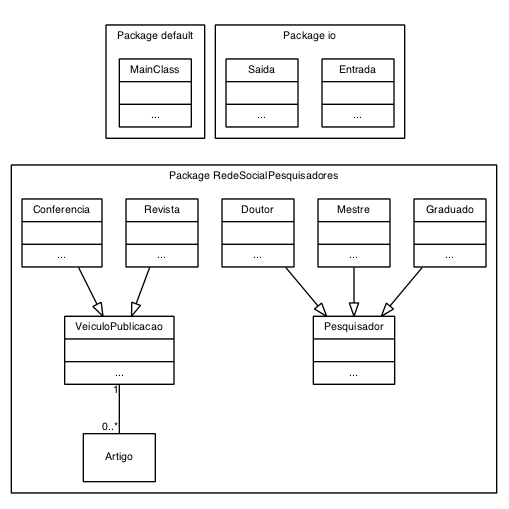
\includegraphics[width=.8\textwidth]{umlsmall.png}
	\caption{Diagrama de classes simplificado}
	\label{uml}
\end{figure}

\begin{figure}[h!]
	\centering
	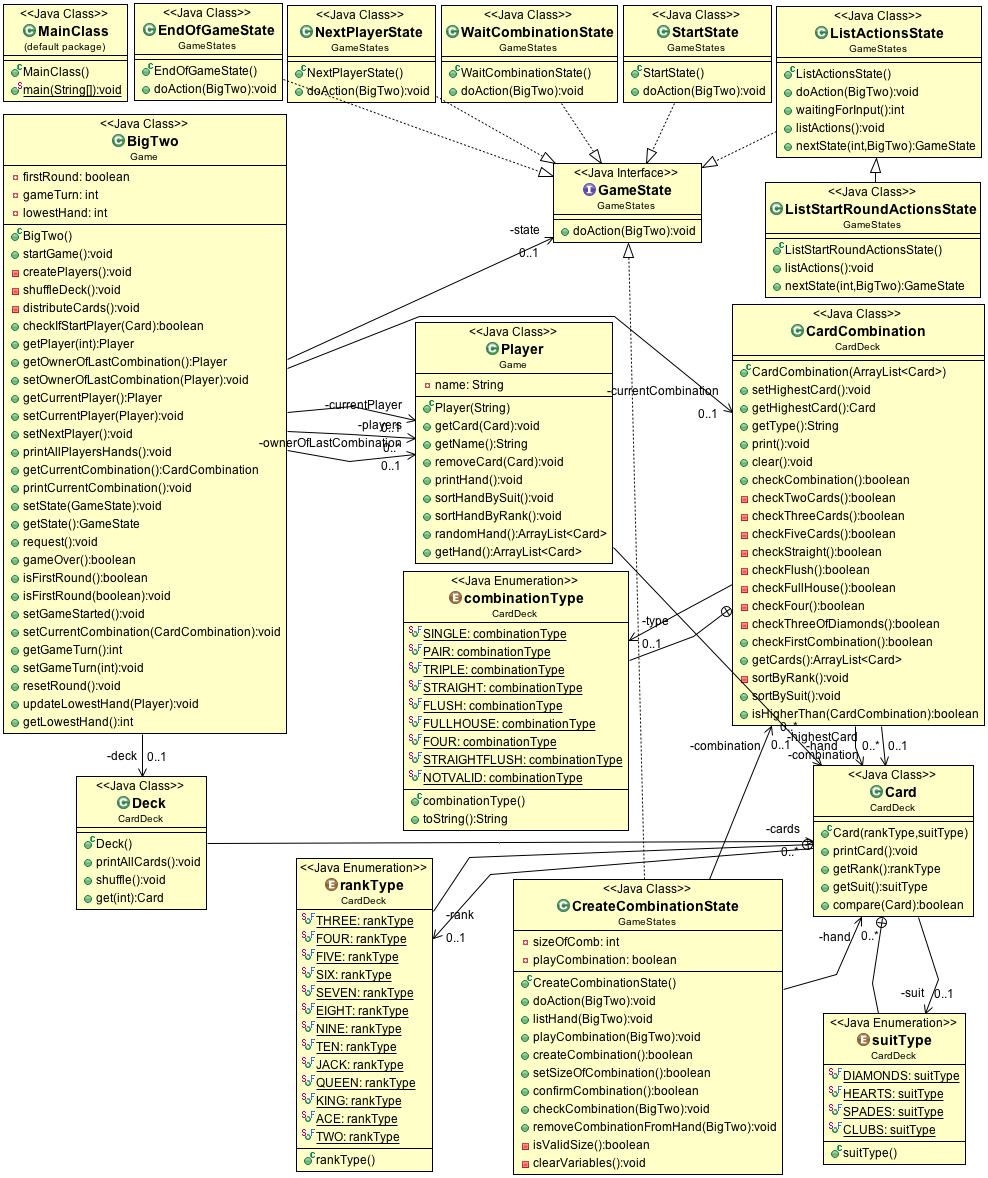
\includegraphics[width=.8\textwidth]{umlfull.png}
	\caption{Diagrama de classes completo}
	\label{umlfull}
\end{figure}


Em resumo, as seguintes classes e subclasses foram criadas:

\section{Classes implementadas}
\vspace{0.2 true cm}
\begin{description}

\item[Pesquisador] \hfill \\
 Classe que contém os dados essenciais de um pesquisador e seus métodos padrões, como \textit{getters}, \textit{setters} além de implementações gerais de certas métricas, como o cálculo de popularidade.
 \vspace{0.01 true cm}
\begin{adjustwidth}{1.2cm}{}
 \item[\textbf{Graduado}] \hfill \\
		Classe filha de Pesquisador. Apenas sobrescreve o método para o cálculo de popularidade.
 \item[\textbf{Mestre}] \hfill \\
		Classe filha de Pesquisador. Sobrescreve método de impressão e de popularidade. Adiciona possibilidade de orientar alunos de graduação.
\item[\textbf{Doutor}] \hfill \\
		Classe filha de Pesquisador. Sobrescreve método de impressão e de popularidade. Permite orientar alunos de graduação, mestrado e doutorado, então vários métodos \textit{getters} e \textit{setters} foram implementados.
\end{adjustwidth}

\vspace{0.2 true cm}

\item[Veículo Publicação] \hfill \\
		Classe que possui dados e métodos padrões de tipos diferentes de veículos de publicação.

\begin{adjustwidth}{1.2cm}{}
\item[\textbf{Revista}] \hfill \\
		Classe filha de Veículo Publicação. Sobrescreve apenas o método de cálculo de valor de impacto.
 \item[\textbf{Conferência}] \hfill \\
		Classe filha de Veículo Publicação. Sobrescreve apenas o método de cálculo de valor de impacto.
\end{adjustwidth}


\item[Artigo] \hfill \\
		Classe que representa artigos, todos seus dados, como, por exemplo, a quantidade de citações que cada um possui.

\item[Entrada] \hfill \\
		Classe que lida com leitura de arquivos.
\item[Saída] \hfill \\
		Classe que lida com escrita de arquivos.
\item[MainClass] \hfill \\
		Class principal que lê arquivos, calcula métricas e escreve o resultado em arquivos de saída.

\end{description}

\subsection{Principais métodos implementados}

Essa subseção irá listar os principais métodos implementados no sistema. Funções triviais não serão listadas, como \textit{getters}, \textit{setters} ou similares. Os métodos detalhados a seguir são os principais utilizados para calcular as métricas solicitadas pelo trabalho prático.


\subsubsection{Pesquisador}

\begin{itemize}
 \item \begin{large}\textit{public double calculaPesoImportancia()}\end{large}\\
 \subitem \textbf{Descrição:} Calcula peso de importância do pesquisador.
 \subitem \textbf{Retorno:} Retorna o resultado no formato \textit{double}.
\end{itemize}

\vspace{0.2 true cm}

\begin{itemize}
 \item \begin{large}\textit{public int totalCitacoes()}\end{large}\\
 \subitem \textbf{Descrição:} Calcula o número de vezes que os artigos do pesquisador foram citados.
 \subitem \textbf{Retorno:} Retorna o resultado no formato \textit{int}.
\end{itemize}

\vspace{0.2 true cm}

\begin{itemize}
 \item \begin{large}\textit{public double calculaPopularidade()}\end{large}\\
 \subitem \textbf{Descrição:} Calcula popularidade do pesquisador, utiliza \textit{calculaPesoImportancia()} e \textit{totalCitacoes()} para realizar o cálculo. É sobrescrita nas classes filhas pois o cálculo irá se especializar.
 \subitem \textbf{Retorno:} Retorna o resultado no formato \textit{double}.
\end{itemize}

\vspace{0.2 true cm}

\subsubsection{Veículo Publicação}

\begin{itemize}
 \item \begin{large}\textit{public int calculaCitacoes()}\end{large}\\
 \subitem \textbf{Descrição:} Calcula o somatório do numero de citações de cada artigo presente em cada veiculo de publicação.
 \subitem \textbf{Retorno:} Retorna o resultado no formato \textit{int}.
\end{itemize}

\vspace{0.2 true cm}

\begin{itemize}
 \item \begin{large}\textit{public double calculaFatorImpacto()}\end{large}\\
 \subitem \textbf{Descrição:} Calcula o fator de impacto do veiculo de publicação, utiliza o \textit{calcularCitacoes() para realizar o cálculo.}. Função é sobrescrita nas classes filhas para especializar o cálculo
 \subitem \textbf{Retorno:} Retorna o resultado no formato \textit{double}.
\end{itemize}

\vspace{0.2 true cm}

\subsubsection{Artigo}

\begin{itemize}
 \item \begin{large}\textit{public double calculaPontuacaoArtigo(ArrayList \textless VeiculoPublicacao\textgreater listaVeiculosPublicacao)}\end{large}\\
 \subitem \textbf{Descrição:} Calcula a pontuação do artigo com base no veículo de publicação e a quantidade de citações do artigo.
 \subitem \textbf{Parâmetros:} Utiliza uma lista com todos os veículos de publicação para encontrar aquele no qual o artigo está associado.
 \subitem \textbf{Retorno:} Retorna o resultado no formato \textit{double}.
\end{itemize}


\section{Testes}
\label{testes}
Realizamos testes utilizando as entradas fornecidas junto com o trabalho. Além disso criamos uma entrada menor para poder anexar junto à esse documento. Essa saída tem como objetivo apenas ilustrar o funcionamento do programa para uma entrada menor do que a fornecida inicialmente.

\subsection{Listagem da saída}

\begin{verbatim}
fatorImpacto_veiculo.txt
1;1.5000
2;1.5000
3;1.8750
4;1.5833

pontuacao_artigo.txt 
1;1.5833
2;1.5000
3;0.0000
4;1.8750
5;1.8750
6;1.5000
7;3.7500
8;1.5000
9;3.1667
10;0.0000
11;0.0000
12;0.0000
13;1.5833
14;0.0000
15;1.8750
16;0.0000
17;0.0000
18;1.8750
19;0.0000
20;0.0000
21;1.8750
22;0.0000
23;1.5000
24;1.5833
25;0.0000
26;1.8750
27;0.0000
28;1.5000
29;1.5000
30;1.8750
31;0.0000
32;1.8750
33;0.0000
34;1.8750
35;0.0000
36;0.0000
37;0.0000
38;0.0000
39;0.0000
40;0.0000
41;0.0000
42;3.0000
43;1.5833
44;3.7500
45;1.5000
46;1.8750
47;1.5000
48;0.0000
49;1.5000
50;1.5833

popularidade_pesquisador.txt 
1;917.7500
2;232.0000
3;325.8333
4;285.0000
5;418.0000
6;317.3333
7;496.3333
8;531.0000
9;320.5000
10;298.3333
11;361.0000
12;375.0000
13;520.0000
14;283.0000
15;314.5000
\end{verbatim}

\section{Conclusão}
\label{conclusao}

O trabalho prático foi prazeroso de ser realizado. Os conceitos de modelagem de classe aprendidos em sala foram bastante reforçados quando nos deparamos com um problema complexo como este.

A maior crítica em relação ao trabalho prático é em relação à mudança de especificações depois do trabalho ter sido lançado. Como ocorreu no nosso grupo, não tínhamos acessado o fórum de discussões até o momento em que nos deparamos com alguma dúvidas em relação à saída. Quando acessamos o fórum vimos que a saída esperada tinha mudado e novos arquivos estavam lá \cite{forum}. 

No fórum também notamos que algumas especificações tinham mudado, como, por exemplo, a passagem dos arquivos de entrada (e saída) como parâmetro para o programa. Nossa sugestão é que caso ocorram mudanças na especificação do trabalho elas devem ser notificadas para todos os alunos de uma outra maneira. Caso contrário precisaremos ler todos os tópicos do fórum com uma certa regularidade para verificar se alguma especificação foi alterada.


\bibliographystyle{sbc}
\bibliography{tp1}

\end{document}
